\documentclass{article}

\usepackage{amsmath,amssymb}
\usepackage{tikz}
\usepackage{pgfplots}
\usepackage{xcolor}
\usepackage[left=2.1cm,right=3.1cm,bottom=3cm,footskip=0.75cm,headsep=0.5cm]{geometry}
\usepackage{enumerate}
\usepackage{enumitem}
\usepackage{marvosym}
\usepackage{tabularx}
\usepackage{tikz-qtree}
\usetikzlibrary{patterns,arrows,calc,decorations.pathmorphing,backgrounds, positioning,fit,petri,decorations.fractals,trees,cd,automata,babel,shapes.geometric,arrows.meta,bending}

\usepackage[utf8]{inputenc}
\usepackage{parskip}

\renewcommand*{\arraystretch}{1.4}

\newcolumntype{L}[1]{>{\raggedright\arraybackslash}p{#1}}
\newcolumntype{R}[1]{>{\raggedleft\arraybackslash}p{#1}}
\newcolumntype{C}[1]{>{\centering\let\newline\\\arraybackslash\hspace{0pt}}m{#1}}

\title{\textbf{Steuertheorie, Hausaufgabe 5}}
\author{\textsc{Henry Haustein}}
\date{}

\begin{document}
	\maketitle
	
	\section*{Aufgabe 1}
	Eine Lohnsteuer verzerrt das Preisverhältnis von Freizeit und Konsum. Der Substitutionseffekt ist negativ bei einer Steuererhöhung, aber der Einkommenseffekt kann den Substitutionseffekt überkompensieren (Einkommen sinkt so stark, dass man mehr arbeiten muss.) Der Substitutionseffekt sorgt dahingehend für Effizienzverlust, dass nun steuerpflichte Leistungen selber gemacht werden (Handwerker $\to$ DIY). Mit einer Pauschalsteuer könnte das gleiche Steueraufkommen erzielt werden, bei höherem Nutzen.
	
	Fall 1: Verringerung des Arbeitsangebotes, Freizeit ist normales Gut: $F\uparrow$, Preis von Freizeit $\downarrow$, Nachfrage $\uparrow$
	
	Fall 2: Ausweitung des Arbeitsangebotes, Freizeit ist ein Giffen-Gut: $F\downarrow$, Preis $\downarrow$, Nachfrage $\downarrow$
	\begin{center}
		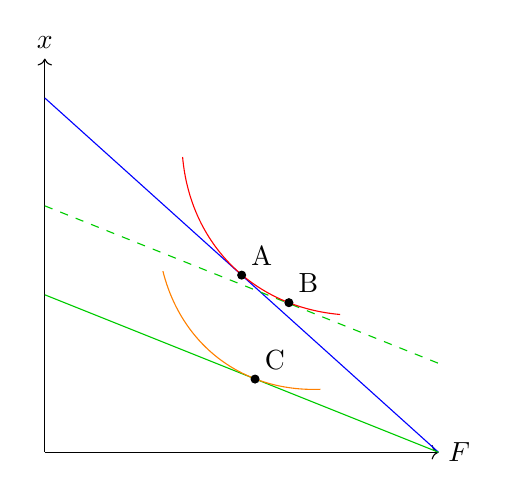
\begin{tikzpicture}
			\draw[->] (0,0) -- (5,0) node[right] {$F$};
			\draw[->] (0,0) -- (0,5) node[above] {$x$};
			
			\draw[blue] (0,4.5) -- (5,0);
			\draw[green!80!black] (0,2) -- (5,0);
			\draw[green!80!black,dashed] (0,3.13) -- (5,1.13);
			
			\draw[red] (1.75,3.75) to[bend right=40] (3.75,1.75);
			\draw[orange] (1.5,2.3) to[bend right=39] (3.5,0.8);
			
			\draw[black,fill=black] (2.5,2.25) circle (0.05) node[above right] {A};
			\draw[black,fill=black] (3.1,1.9) circle (0.05) node[above right] {B};
			\draw[black,fill=black] (2.67,0.93) circle (0.05) node[above right] {C};
		\end{tikzpicture} \\
		Fall 1, \textcolor{blue}{Budgetrestriktion ohne Steuer}, \textcolor{green!80!black}{Budgetrestriktion mit Steuer}, \textcolor{red}{Nutzen ohne Steuer}, \textcolor{orange}{Nutzen ohne Steuer}
	\end{center}
	\begin{center}
		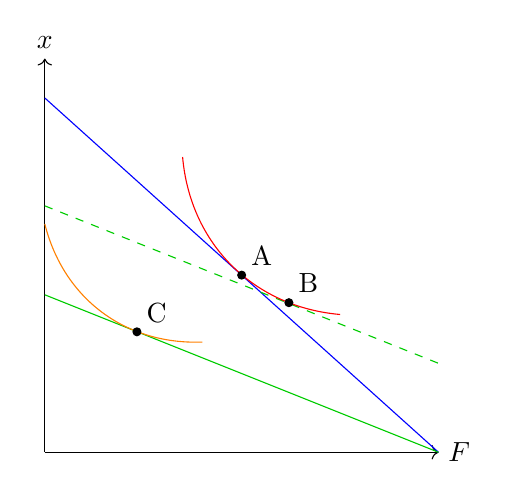
\begin{tikzpicture}
			\draw[->] (0,0) -- (5,0) node[right] {$F$};
			\draw[->] (0,0) -- (0,5) node[above] {$x$};
			
			\draw[blue] (0,4.5) -- (5,0);
			\draw[green!80!black] (0,2) -- (5,0);
			\draw[green!80!black,dashed] (0,3.13) -- (5,1.13);
			
			\draw[red] (1.75,3.75) to[bend right=40] (3.75,1.75);
			\draw[orange] (0,2.9) to[bend right=39] (2,1.4);
			
			\draw[black,fill=black] (2.5,2.25) circle (0.05) node[above right] {A};
			\draw[black,fill=black] (3.1,1.9) circle (0.05) node[above right] {B};
			\draw[black,fill=black] (1.17,1.53) circle (0.05) node[above right] {C};
		\end{tikzpicture} \\
		Fall 2, \textcolor{blue}{Budgetrestriktion ohne Steuer}, \textcolor{green!80!black}{Budgetrestriktion mit Steuer}, \textcolor{red}{Nutzen ohne Steuer}, \textcolor{orange}{Nutzen ohne Steuer}
	\end{center}
	Der Substitutionseffekt ist von A $\to$ B und der Einkommenseffekt ist von B $\to$ C
	
	\section*{Aufgabe 2}
	\begin{enumerate}[label=(\alph*)]
		\item Die Budgetrestriktion für den Haushalt ist
		\begin{align}
			wL_i &= px_i + T_i \notag \\
			T_i &= a_i\cdot L_i - b_i \notag \\
			L_i &= x_i + a_i\cdot L_i - b_i \notag \\
			x_i &= L_i(1-a_i) + b_i \notag
		\end{align}
		Der Lagrange-Ansatz zur Maximierung des Nutzens liefert
		\begin{align}
			\mathcal{L} &= 4x_i - c_i\cdot L^2 + \lambda(L(1-a_i)+b_i-x_i) \notag
		\end{align}
		Die Bedingungen erster Ordnung lauten
		\begin{align}
			\frac{\partial\mathcal{L}}{\partial x_i} &= 4-\lambda =0 \notag \\
			\lambda &= 4 \notag \\
			\frac{\partial\mathcal{L}}{\partial L_i} &= -2c_i\cdot L_i + \lambda(1-a_i) =0 \notag \\
			2c_i\cdot L_i &= 4(1-a_i) \notag \\
			L_i &= \frac{2(1-a_i)}{c_i} \notag
		\end{align}
		Das Steueraufkommen ist
		\begin{align}
			\mathcal{T} &= \sum_{i=L,H} a_i\cdot L_i \notag \\
			&= \sum_{i=L,H} a_i\cdot\frac{2(1-a_i)}{c_i} \notag
		\end{align}
		Die Änderungen von Arbeitsangebot und Steueraufkommen mit Änderung der Steuer sind
		\begin{align}
			\frac{\partial L_i}{a_i} &= -\frac{2}{c_i} \quad(\text{Wenn die Steuer erhöht wird, sinkt das Arbeitsangebot}) \notag \\
			\frac{\partial \mathcal{T}}{\partial a_i} &= \sum_{i=L,H} \left(\frac{2(1-a_i)}{c_i} - a_i\cdot\frac{2}{c_i}\right) \notag \\
			&= \sum_{i=L,H} \frac{2(1-2a_i)}{c_i} \notag
		\end{align}
		Das Maximum des Steueraufkommens ist also bei $a_i=\frac{1}{2}$; das Steueraukommen steigt wenn $a_i<\frac{1}{2}$ und sinkt, wenn $a_i>\frac{1}{2}$.
		\item Für einen Haushalt gilt
		\begin{align}
			x_i &= (1-a_i)L_i + b_i \notag \\
			L_i &= \frac{2(1-a_i)}{c_i} \notag \\
			x_i &= \frac{2(1-a_i)^2}{c_i} + b_i \notag \\
			U_i &= 4x_i - c_i\cdot L^2 \notag \\
			&= \frac{8(1-a_i)^2}{c_i} + 4b_i - c_i\cdot\frac{4(1-a_i)^2}{c_i^2} \notag \\
			&= \frac{4(1-a_i)^2}{c_i}-4b_i \notag
		\end{align}
		Der Staat möchte ein ausgeglichenes Budget, also
		\begin{align}
			a_H\cdot L_H + a_L\cdot L_L &= b_H + b_L \notag \\
			a_H\cdot\frac{2(1-a_H)}{c_H} + a_L\cdot\frac{2(1-a_L)}{c_L} &= b_H + b_L \notag
		\end{align}
		Der Lagrange-Ansatz liefert
		\begin{align}
			\mathcal{L} &= \sqrt{U_L} + \sqrt{U_H} + \lambda\left(a_H\cdot\frac{2(1-a_H)}{c_H} + a_L\cdot\frac{2(1-a_L)}{c_L} - b_H - b_L\right) \notag \\
			&= \sqrt{\frac{4(1-a_L)^2}{c_L}-4b_L} + \sqrt{\frac{4(1-a_H)^2}{c_H}-4b_H} + \lambda\left(a_H\cdot\frac{2(1-a_H)}{c_H} + a_L\cdot\frac{2(1-a_L)}{c_L} - b_H - b_L\right) \notag
		\end{align}
		Die Bedingungen erster Ordnung lauten
		\begin{align}
			\frac{\partial\mathcal{L}}{\partial a_i} &= \frac{1}{2\sqrt{\frac{4(1-a_i)^2}{c_i}-4b_i}} \cdot -\frac{8(1-a_i)}{c_i} + \lambda\left(\frac{2-4a_i}{c_i}\right) = 0 \notag \\
			\label{2.1}
			\lambda\left(\frac{2-4a_i}{c_i}\right) &= \frac{1}{2\sqrt{\frac{4(1-a_i)^2}{c_i}-4b_i}} \cdot \frac{8(1-a_i)}{c_i} \tag{2.1} \\
			\frac{\partial\mathcal{L}}{\partial b_i} &= \frac{1}{2\sqrt{\frac{4(1-a_i)^2}{c_i}-4b_i}}\cdot 4-\lambda = 0 \notag \\
			\label{2.2}
			\lambda &= \frac{1}{2\sqrt{\frac{4(1-a_i)^2}{c_i}-4b_i}}\cdot 4 \tag{2.2} \\
			\frac{\partial\mathcal{L}}{\partial\lambda} &= a_H\cdot\frac{2(1-a_H)}{c_H} + a_L\cdot\frac{2(1-a_L)}{c_L} - b_H - b_L \notag \\
			\label{2.3}
			b_H + b_L &= a_H\cdot\frac{2(1-a_H)}{c_H} + a_L\cdot\frac{2(1-a_L)}{c_L} \tag{2.3}
		\end{align}
		Division von \eqref{2.1} durch \eqref{2.2} ergibt
		\begin{align}
			\frac{\frac{1}{2\sqrt{\frac{4(1-a_i)^2}{c_i}-4b_i}} \cdot \frac{8(1-a_i)}{c_i}}{\frac{1}{2\sqrt{\frac{4(1-a_i)^2}{c_i}-4b_i}}\cdot 4} &= \frac{\lambda\left(\frac{2-4a_i}{c_i}\right)}{\lambda} \notag \\
			\frac{2-2a_i}{c_i} &= \frac{2-4a_i}{c_i} \notag \\
			2-2ai &= 2-4a_i \notag \\
			2a_i &= 0 \notag \\
			a_i &= 0 \notag
		\end{align}
		Einsetzen in \eqref{2.3}:
		\begin{align}
			b_H + b_L &= 0\cdot\frac{1-0}{c_H} + 0\cdot\frac{1-0}{c_L} \notag \\
			b_H &= -b_L \notag
		\end{align}
		Aus \eqref{2.2} sehen wir, dass $\lambda=\frac{1}{2\sqrt{U_i}}\cdot 4$ gilt, insbesondere gilt das sowohl für $i=L$ als auch für $i=H$. Das lässt den Schluss zu, dass $U_L=U_H$ gilt und damit folgt
		\begin{align}
			U_H &= U_L \notag \\
			\frac{4(1-0)^2}{\frac{1}{8}} + 4b_H &= \frac{4(1-0)^2}{\frac{1}{4}} + 4b_L \notag \\
			32 + 4b_H &= 16 + 4b_L \notag \\
			32 - 4b_L &= 16 + 4b_L \notag \\
			16 &= 8b_L \notag \\
			b_L &= 2 \Rightarrow b_H = -2 \notag
		\end{align}
		Die Grenzsteuersätze sind 0 und die Umverteilung läuft über Pauschalsteuern. $H$ zahlt eine Steuer, die $L$ als Transfer bekommt.
		\item Es ist für den Staat nicht beobachtbar, ob ein Haushalt $H$ oder $L$ ist, er sieht nur den Verdienst. Damit besteht für $H$-Haushalte ein Anreiz sich als $L$-Haushalte auszugeben, um den Transfer zu erhalten. $H$-Haushalte reduzieren das Arbeitsangebot, wobei das geringere Konsumniveau über einen höheren Freizeitkonsum mehr als kompensiert wird $\Rightarrow$ nicht anreizkompatibel.
	\end{enumerate}

	\section*{Aufgabe 3}
	\begin{enumerate}[label=(\alph*)]
		\item Das Einkommen $y_i=w_i\cdot L_i$ und damit $L_i=\frac{y_i}{w_i}$. Einsetzen in die Nutzenfunktion liefert
		\begin{align}
			U_i &= u(x_i) + v\left(\frac{y_i}{w_i}\right) \notag
		\end{align}
		Das totale Differential ist $u_{x_i}\cdot dx_i + v_A\cdot\frac{1}{w_i}\cdot dy_i$ und damit
		\begin{align}
			\frac{dx_i}{dy_i}\bigg\vert_{\bar{U}} &= -\frac{\frac{v_A}{w_i}}{u_{x_i}} >0 \notag
		\end{align}
		da $v'<0$ und $u'>0$.
		\item Wir wissen, dass $w_L<w_H$ und damit folgt
		\begin{align}
			\frac{dx_L}{dy_L}\bigg\vert_{\bar{U}} = \frac{\frac{v_A}{w_L}}{u_{x_L}} > \frac{\frac{v_A}{w_H}}{u_{x_H}} = \frac{dx_H}{dy_H}\bigg\vert_{\bar{U}} \notag
		\end{align}
		\item Der Staat maximiert $U_H(x_H,y_H)$ unter den Nebenbedingungen
		\begin{align}
			\label{3.1}
			U^L(x^L,y^L) &\ge \bar{U}^L \tag{3.1} \\
			\label{3.2}
			U^H(x^H,x^H) &\ge U^H(x^L,y^L) \tag{3.2} \\
			\label{3.3}
			(y^H-x^H)\cdot N^H + (y^L-x^L)\cdot N^L &\ge 0 \tag{3.3}
		\end{align}
		\begin{itemize}
			\item \eqref{3.1} garantiert den $L$-Typen mindestens das Nutzenniveau $\bar{U}^L$.
			\item \eqref{3.2} besagt, dass die $H$-Typen keinen Anreiz haben dürfen, sich als $L$-Typen auszugeben (Selbstselektionsbedingung).
			\item \eqref{3.3} ist die Budgetrestriktion des Staates.
		\end{itemize}
		\item Lagrange
		\begin{align}
			\mathcal{L} &= U^H(x^H,y^H) + \mu\left(U^L(x^L,y^L) - \bar{U}^L\right) + \lambda\left(U^H(x^H,x^H) - U^H(x^L,y^L)\right) \notag \\
			&+ \gamma\left((y^H-x^H)\cdot N^H + (y^L-x^L)\cdot N^L\right) \notag
		\end{align}
		Bedingungen erster Ordnung
		\begin{align}
			\label{3.4}
			\frac{\partial \mathcal{L}}{\partial x^H} &= \frac{\partial U^H}{\partial x^H} + \lambda\frac{\partial U^H}{\partial x^H} - \gamma N^H =0 \tag{3.4} \\
			\label{3.5}
			\frac{\partial \mathcal{L}}{\partial y^H} &= \frac{\partial U^H}{\partial y^H} + \lambda\frac{\partial U^H}{\partial y^H} + \gamma N^H =0 \tag{3.5} \\
			\label{3.6}
			\frac{\partial \mathcal{L}}{\partial x^L} &= \mu\frac{\partial U^L}{\partial x^L} - \lambda\frac{\partial U^L}{\partial x^L} - \gamma N^L =0 \tag{3.6} \\
			\label{3.7}
			\frac{\partial \mathcal{L}}{\partial y^L} &= \mu\frac{\partial U^L}{\partial y^L} - \lambda\frac{\partial U^L}{\partial y^L} + \gamma N^L =0 \tag{3.7}
		\end{align}
		Division von \eqref{3.5} durch \eqref{3.4} ergibt
		\begin{align}
			-\frac{\frac{\partial U^H}{\partial y^H}}{\frac{\partial U^H}{\partial x^H}} = 1 \notag
		\end{align}
		Die linke Seite entspricht der Grenzrate der Substitution:
		\begin{align}
			\frac{dx^H}{dy^H}\bigg\vert_{\bar{U}} = 1 \notag
		\end{align}
		Mit jedem Euro mehr Einkommen steigt auch der Konsum um einem Euro $\Rightarrow$ Grenzsteuersatz 0. Der Durchschnittsteuersatz muss natürlich positiv sein, da von den Hochproduktiven die Steuer erhoben wird, mit der die Transfers an die gering Produktiven finanziert werden.
	\end{enumerate}
	
\end{document}